\begin{minipage}[t]{180mm}
\fcolorbox{black}{white}{
\begin{minipage}[b]{30mm}

\includegraphics[width=0.5\linewidth]{unflogo.pdf}
\end{minipage}
\begin{minipage}[b]{100mm}
\Huge \textbf{UNF NEWZ} \\
\Large -- Søvn og retsstavning er overvurderet! 
\end{minipage}
\begin{minipage}[b]{50mm}
\Large Onsdag 17.07.2015 \\
\normalsize Redigeret i \LaTeX\ af \\ SOM, MGS, MMN, SABH
\end{minipage}
}
\end{minipage}



\begin{minipage}[b]{0.95\linewidth}
\begin{minipage}[t]{0.47\textwidth}
\vspace{3mm}
\section*{Vi tager bestik af situationen}

5 grunde til, hvorfor bestikket i bestikskuffen skal ligge i rækkefølgen ske, gaffel, kniv fra venstre:

\begin{itemize}
\item Fordi det er godt at have standardiseret rækkefølgen, så man altid ved, hvor man skal finde det ønskede bestik
\item Fordi kniven skal ligge til højre for gaflen
\item Fordi de fleste mennesker er højrehåndede, og de skal nå at skære/stikke sig på flest mulige ting i skuffen
\item Fordi man ikke kan have, at det sker, at det kniber med gaflerne, men det må godt ske, at man gafler en kniv
\item Fordi jeg har CDO (det er ligesom OCD, bogstaverne er bare ordnet alfabetisk – som de bør være)
\end{itemize}

\section*{Produktanmeldelse -- }


\vspace{1mm}
\section*{Madanmeldelse -- }
\fcolorbox{black}{white}{$x$ ud af $\aleph_3$ chokoladekiks}


\end{minipage}%
\hfill\begin{minipage}[t]{0.47\textwidth}
\vspace{3mm}
\section*{Vejrudsigt}
\textbf{IMF, AU (fra DMI)}: Temperaturer fra 14 til 23 grader og tørvejr med en del sol indtil midt om eftermiddagen. Der forventes et moderat antal græspollen, og et lavt antal bynkepollen.

\textbf{SEN/ASN}: Solskin og 26 grader, men nogle skyer. Ludtfugtighed på cirka 90 \% og ingen vind.

\vspace{-2mm}
\section*{Dagens statistiker}
Hvis du møder en statistiker, så prik hende, og forklar at hun ikke er signifikant.

\vspace{-2mm}
\section*{Find en Fynbo}

\vspace{-2mm}
\section*{Fakta om Jylland}
JYLLAND er i virkeligheden en forkortelse for Jernalderens Yderst Lovlige og Legitime Arbejderes Nydannede Danmark.

\vspace{-2mm}
\section*{Dagens sandsynlighed}

\vspace{1mm}
%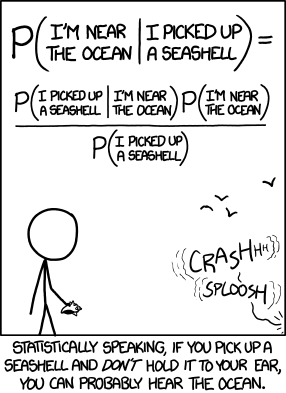
\includegraphics[width=95mm]{seashell.png}
\tiny Randall Munroe, http://xkcd.com/1236/, CC-BY-SA-2.5
\end{minipage}

\begin{center}
\tiny UNF Newz er avisen hvor at ansvarshavende redaktør fralægger sig ethvert ansvar for eventuel plagiering, kaniner, tysk, stavefelj, kaffe, dårlig humor, glemsomhed, katte, store sigmaer, pile, skyer, dårlige oversættelser og alt hvad eventuelle homo sapiens sapiens kunne finde på at holde imod UNF Newz! Dog tager UNF Newz fuld credit og copyright for alle guldkorn, magickort, mus, \TeX, humor, smil, Mortener, kaffe, før-fremtid, ringe og/eller rubik's cube.
\end{center}
\end{minipage}

